% Team talk: A Forensic Pipeline for Standardized Foundation Model Evaluation via BPB
% Target: 10 minutes. Build with:  pdflatex -interaction=nonstopmode talk.tex  (twice)
\documentclass[aspectratio=169,11pt]{beamer}

\usepackage[utf8]{inputenc}
\usepackage[T1]{fontenc}
\usepackage[scaled=0.92]{helvet}
\renewcommand{\familydefault}{\sfdefault}
\usepackage{amsmath,amssymb}
\usepackage{booktabs}
\usepackage{graphicx}
\usepackage{tikz}
\usepackage{xcolor}
\usepackage{colortbl}
\usepackage{microtype}
\usetikzlibrary{calc, positioning, arrows.meta, fit, backgrounds}

\graphicspath{{../figures/}{figures/}}

% ---------------------------------------------------------------- theme
\usetheme{default}
\usecolortheme{default}
\setbeamertemplate{navigation symbols}{}

\definecolor{ink}{HTML}{1C2733}
\definecolor{accent}{HTML}{3B6FA0}
\definecolor{warm}{HTML}{C07C33}
\definecolor{good}{HTML}{3F8457}
\definecolor{mute}{HTML}{6B7785}
\definecolor{rule}{HTML}{D7DDE4}
\definecolor{wash}{HTML}{F4F6F8}

\setbeamercolor{normal text}{fg=ink}
\setbeamercolor{frametitle}{fg=ink}
\setbeamercolor{structure}{fg=accent}
\setbeamercolor{itemize item}{fg=accent}
\setbeamercolor{itemize subitem}{fg=mute}
\setbeamerfont{frametitle}{size=\large,series=\bfseries}
\setbeamerfont{framesubtitle}{size=\small,series=\mdseries}
\setbeamercolor{framesubtitle}{fg=mute}
\setbeamertemplate{itemize item}{\raisebox{0.18ex}{\scriptsize$\blacksquare$}}
\setbeamertemplate{itemize subitem}{\textendash}
\setbeamertemplate{caption}{\insertcaption}
\setlength{\leftmargini}{1.4em}

% frame title with a hairline under it
\makeatletter
\setbeamertemplate{frametitle}{%
  \vspace{0.9em}%
  \begin{beamercolorbox}[wd=\paperwidth,leftskip=0.9cm,rightskip=0.9cm]{frametitle}%
    \usebeamerfont{frametitle}\insertframetitle%
    \ifx\insertframesubtitle\@empty\else%
      \\[0.15em]{\usebeamerfont{framesubtitle}\usebeamercolor[fg]{framesubtitle}\insertframesubtitle}%
    \fi%
    \\[0.35em]{\color{rule}\rule{\dimexpr\paperwidth-1.8cm\relax}{0.6pt}}%
  \end{beamercolorbox}%
  \vspace{-0.2em}%
}
\makeatother

% slide number, bottom right
\setbeamertemplate{footline}{%
  \hfill{\color{mute}\scriptsize\insertframenumber}\hspace{0.9cm}\vspace{0.35cm}%
}

% ---------------------------------------------------------------- helpers
\newcommand{\bpb}{\textsc{bpb}}
\newcommand{\ppl}{\textsc{ppl}}
\newcommand{\keyw}[1]{\textcolor{accent}{\textbf{#1}}}
\newcommand{\warmw}[1]{\textcolor{warm}{\textbf{#1}}}
\newcommand{\goodw}[1]{\textcolor{good}{\textbf{#1}}}

% rank-displacement markers for the BPB-vs-static ordering table.
% \up{n} = ranks n places HIGHER on this benchmark than on BPB (benchmark flatters it)
% \dn{n} = ranks n places LOWER
\newcommand{\up}[1]{\,{\color{good}\scriptsize$\blacktriangle$#1}}
\newcommand{\dn}[1]{\,{\color{warm}\scriptsize$\blacktriangledown$#1}}
\newcommand{\same}{\,{\color{mute}\scriptsize$\bullet$}}

% suppress hyphenation inside narrow boxes -- avoids ugly mid-word breaks
\newcommand{\nohyph}{\hyphenpenalty=10000\exhyphenpenalty=10000\raggedright}

% a soft callout band
\newcommand{\punch}[1]{%
  \begin{center}%
  \begin{minipage}{0.92\textwidth}%
    \setlength{\fboxsep}{9pt}%
    \colorbox{wash}{\parbox{\dimexpr\textwidth-2\fboxsep\relax}{\nohyph #1}}%
  \end{minipage}%
  \end{center}%
}

% ---------------------------------------------------------------- title
\title{\textbf{Beyond perplexity}}
\subtitle{Entropy-based evaluation of base language models}
\author{David Afonso Valente}
\institute{Bottlecap AI}
\date{August 2026}

\begin{document}

% ==================================================================== 1
{
\setbeamertemplate{footline}{}
\begin{frame}[plain]
  \vspace{1.2em}
  {\color{rule}\rule{\textwidth}{0.8pt}}\\[1.1em]
  {\LARGE\bfseries Beyond perplexity}\\[0.55em]
  {\large\color{mute} Entropy-based evaluation of base language models}\\[1.1em]
  {\color{rule}\rule{\textwidth}{0.8pt}}\\[1.4em]
  {\small\textbf{David Afonso Valente} \quad\textcolor{mute}{$\cdot$}\quad Bottlecap AI}\\[0.3em]
  {\small\color{mute} August 2026 \quad$\cdot$\quad under 10 minutes}
\end{frame}
}

% ==================================================================== 2
\begin{frame}
  \frametitle{Return to the language-modeling objective}
  \framesubtitle{Fixed benchmarks are useful slices, not a complete measure of a base model}

  \vspace{0.4em}
  \begin{columns}[t]
  \begin{column}{0.47\textwidth}
    \keyw{Perplexity stopped comparing fairly}\\[0.6em]
    \small
    \ppl{} is measured \emph{per token}, but each model divides text differently:
    Llama-3.2 has \textbf{128,000} vocabulary entries and Qwen-2.5 has \textbf{151,643}.
    \vspace{0.6em}

    \bpb{} divides loss by UTF-8 bytes. A byte is the same amount of text for every model,
    so the scores share one unit.
  \end{column}
  \begin{column}{0.47\textwidth}
    \keyw{Fixed benchmarks have blind spots}\\[0.6em]
    \small
    Task suites sample specific abilities, and repeated optimization on fixed tests makes
    contamination and benchmark-specific tuning harder to separate from general LM quality.
    \vspace{0.6em}

    Entropy sees the full predictive distribution, but it needs a fair denominator, fresh
    target-domain text, and a contamination audit.
  \end{column}
  \end{columns}

  \vspace{0.2em}
  \punch{Go full circle: measure entropy again---with byte normalization, dynamic
  target-domain evaluation, controlled adaptation, and contamination filtering.}
\end{frame}

% ==================================================================== 3
\begin{frame}
  \frametitle{Measure the model we will actually use}
  \framesubtitle{A controlled adaptation turns evaluation into a deployment measurement}

  \vspace{1.0em}
  \begin{center}
  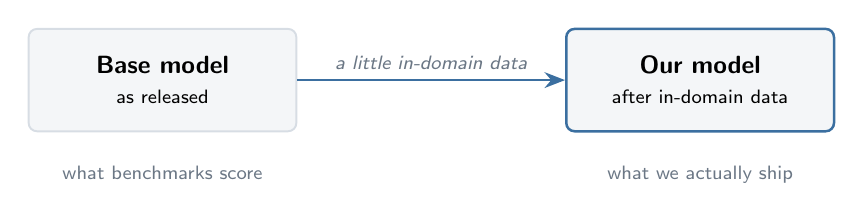
\begin{tikzpicture}[font=\small, >={Stealth[length=2.6mm,width=2.0mm]}]
    \node[align=center, draw=rule, line width=0.7pt, rounded corners=3pt,
          fill=wash, minimum width=3.4cm, minimum height=1.3cm] (a)
      {\textbf{Base model}\\{\scriptsize as released}};
    \node[align=center, draw=accent, line width=0.9pt, rounded corners=3pt,
          fill=wash, minimum width=3.4cm, minimum height=1.3cm, right=3.4cm of a] (b)
      {\textbf{Our model}\\{\scriptsize after in-domain data}};
    \draw[->, line width=1.0pt, draw=accent] (a) -- node[above, font=\scriptsize\itshape, text=mute]
      {a little in-domain data} (b);
    \node[below=0.30cm of a, font=\scriptsize, text=mute] {what benchmarks score};
    \node[below=0.30cm of b, font=\scriptsize, text=mute] {what we actually ship};
  \end{tikzpicture}
  \end{center}

  \vspace{0.9em}
  A benchmark describes the model as released. A product uses the model after domain data.
  We measure both states on the same held-out corpus.

  \vspace{0.5em}
  \punch{The \keyw{adapted BPB level} selects the model. The reduction from zero-shot BPB
  explains how much calibration it needed.}
\end{frame}

% ==================================================================== 4
\begin{frame}
  \frametitle{Two measurements, one decision}

  \vspace{0.8em}
  \begin{columns}[t]
  \begin{column}{0.47\textwidth}
    \keyw{1 --- Use a fair ruler}\\[0.7em]
    Normalize cross-entropy onto \emph{bytes} instead of tokens:
    \vspace{0.3em}
    \[
      \bpb \;=\; \frac{\mathcal{L}_{\text{nats}}}{\ln 2}\times\frac{|\text{tokens}|}{|\text{bytes}|}
    \]
    \vspace{0.1em}

    UTF-8 bytes are the same unit for every model, so \bpb{} is
    \goodw{tokenizer-agnostic}. Same physical text, same denominator, comparable
    numbers.
    \vspace{0.4em}

    {\scriptsize\color{mute} Not ours --- The Pile, Paloma. Under-used, and we make it the primary metric.}
  \end{column}
  \begin{column}{0.47\textwidth}
    \keyw{2 --- Measure domain fit}\\[0.7em]
    For each model, on one identical corpus:
    \vspace{0.5em}
    \begin{enumerate}[1.]\setlength\itemsep{0.35em}
      \item Zero-shot \bpb{}
      \item A \emph{tuned} LoRA adaptation step
      \item Adapted \bpb{}
    \end{enumerate}
    \vspace{0.7em}
    \textbf{Primary output:} adapted \bpb{} for model selection.\\[0.45em]
    \textbf{Diagnostic:} relative reduction for corpus calibration.
  \end{column}
  \end{columns}
\end{frame}

% OPTIONAL IN THE 10-MINUTE PATH (adds 0:37)
% ==================================================================== 5
\begin{frame}
  \frametitle{The pipeline}
  \framesubtitle{Chronologically strict: nothing is scored before it clears the gate}

  \vspace{0.9em}
  \begin{center}
  \resizebox{0.98\textwidth}{!}{
  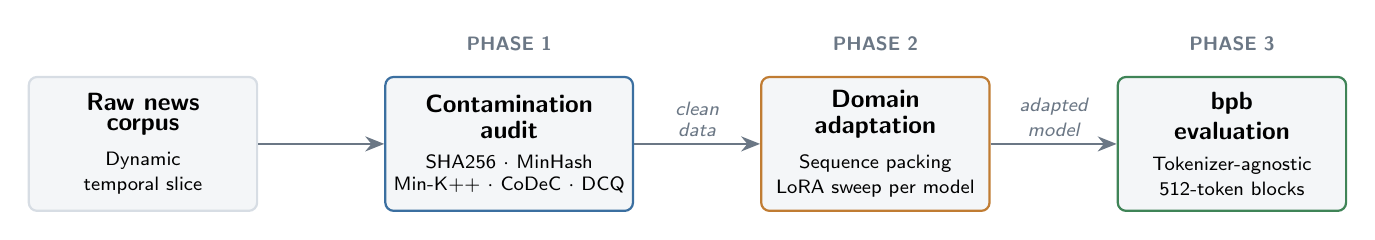
\begin{tikzpicture}[
      font=\small,
      >={Stealth[length=2.4mm,width=1.9mm]},
      stage/.style={draw, line width=0.8pt, rounded corners=3pt,
                    minimum width=2.9cm, minimum height=1.7cm,
                    align=center, inner sep=3pt},
      phase/.style={font=\scriptsize\bfseries, text=mute},
      elbl/.style={font=\scriptsize\itshape, text=mute, fill=white, inner sep=1.5pt},
      flow/.style={->, line width=1.0pt, draw=mute}
  ]
    \node[stage, fill=wash, draw=rule] (data)
      {\shortstack{\textbf{Raw news}\\\textbf{corpus}\\[3pt]{\scriptsize Dynamic}\\{\scriptsize temporal slice}}};
    \node[stage, fill=wash, draw=accent, right=1.6cm of data] (audit)
      {\shortstack{\textbf{Contamination}\\\textbf{audit}\\[3pt]{\scriptsize SHA256 $\cdot$ MinHash}\\{\scriptsize Min-K++ $\cdot$ CoDeC $\cdot$ DCQ}}};
    \node[stage, fill=wash, draw=warm, right=1.6cm of audit] (adapt)
      {\shortstack{\textbf{Domain}\\\textbf{adaptation}\\[3pt]{\scriptsize Sequence packing}\\{\scriptsize LoRA sweep per model}}};
    \node[stage, fill=wash, draw=good, right=1.6cm of adapt] (eval)
      {\shortstack{\textbf{\bpb{}}\\\textbf{evaluation}\\[3pt]{\scriptsize Tokenizer-agnostic}\\{\scriptsize 512-token blocks}}};
    \node[phase, above=2mm of audit] {PHASE 1};
    \node[phase, above=2mm of adapt] {PHASE 2};
    \node[phase, above=2mm of eval]  {PHASE 3};
    \draw[flow] (data)  -- (audit);
    \draw[flow] (audit) -- node[elbl, above=0.2mm]{\shortstack{clean\\data}} (adapt);
    \draw[flow] (adapt) -- node[elbl, above=0.2mm]{\shortstack{adapted\\model}} (eval);
  \end{tikzpicture}}
  \end{center}

  \vspace{0.7em}
  \small
  \textbf{Corpus:} one deduplicated slice of Google News, 8 June 2026 (119k articles),
  split 80/10/10 with zero intersection between splits. \textbf{Cohort:} 11 base models,
  0.5B--35B, dense Transformers $+$ a sparse MoE $+$ a Liquid architecture.
\end{frame}

% OPTIONAL IN THE 10-MINUTE PATH (adds 0:44)
% ==================================================================== 6
\begin{frame}
  \frametitle{Phase 1: why we trust the numbers}
  \framesubtitle{``Scout, then verify'' --- cheap detectors propose, an expensive test decides}

  \vspace{0.8em}
  \begin{columns}[t]
  \begin{column}{0.60\textwidth}
    \small
    \begin{itemize}\setlength\itemsep{0.5em}
      \item \keyw{Min-K++} \textcolor{mute}{(scout)} --- inspect the least-likely 20\% of
      tokens; high confidence on rare tokens looks like recall, not prediction.
      \item \keyw{CoDeC} \textcolor{mute}{(scout, ours)} --- supply the preceding context;
      memorized text shows a non-linear \emph{spike} in confidence.
      \item \keyw{Dynamic Choice Quiz} \textcolor{mute}{(gatekeeper)} --- hide the real
      passage among 16 synthetic near-duplicates. If the model reliably picks the original,
      quarantine it.
    \end{itemize}
    \vspace{0.9em}
    {\footnotesize This rules out benchmark memory as the explanation for an adaptation gain.}
  \end{column}
  \begin{column}{0.36\textwidth}
    \setlength{\fboxsep}{9pt}
    \colorbox{wash}{\parbox{\dimexpr\textwidth-2\fboxsep\relax}{%
      \small\nohyph
      Run \textbf{per model}; we quarantine the \textbf{union} of every model's verified
      leaks.\\[0.7em]
      $\Rightarrow$ all 11 models are adapted and scored on \goodw{one identical,
      cleansed corpus}.\\[0.7em]
      \textbf{80} sequences removed globally.
    }}
  \end{column}
  \end{columns}
\end{frame}

% ==================================================================== 7
\begin{frame}
  \frametitle{Results: 11 models, one ruler}
  \framesubtitle{Grey $=$ as released, blue $=$ after adaptation. Left is better.}

  \vspace{0.2em}
  \begin{columns}[c]
  \begin{column}{0.62\textwidth}
    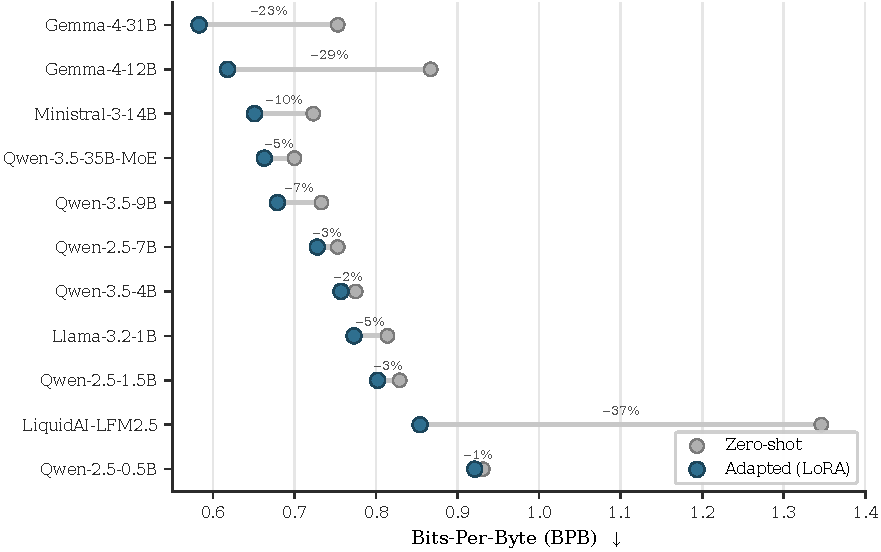
\includegraphics[width=\textwidth]{fig_adaptation.pdf}
  \end{column}
  \begin{column}{0.35\textwidth}
    \small
    \keyw{Gemma-4-31B} reaches the best adapted \bpb{}: \textbf{0.583}.\\[0.6em]
    The \keyw{35B MoE} lands with dense 12--14B models, giving a direct quality measurement
    between its active and total parameter counts.
    \vspace{0.9em}

    \keyw{LFM-2.5} shows the largest calibration shift: \textbf{36.5\%}.
    \vspace{0.7em}

    \textbf{Selection uses the blue endpoint.} Line length explains how much each base
    distribution moved toward the corpus.
  \end{column}
  \end{columns}
\end{frame}

% ==================================================================== 8
\begin{frame}
  \frametitle{Two numbers, two jobs}
  \framesubtitle{The level chooses a model; the reduction explains calibration}

  \vspace{0.9em}
  \begin{columns}[t]
  \begin{column}{0.46\textwidth}
    \keyw{Adapted BPB}\\[0.6em]
    \small
    The primary selection score: how efficiently the adapted model predicts held-out
    target-domain text.
    \vspace{0.7em}

    \goodw{Lower is better.} It is directly comparable across tokenizers and architectures.
  \end{column}
  \begin{column}{0.46\textwidth}
    \keyw{Relative reduction}\\[0.6em]
    \small
    A diagnostic: how much the released model recalibrates to the corpus's style,
    formatting, and context pattern.
    \vspace{0.7em}

    It explains the trajectory; it does not replace the adapted endpoint.
    \vspace{0.7em}

    \textbf{Token-level evidence makes that interpretation visible.}
  \end{column}
  \end{columns}
\end{frame}

% ==================================================================== 9
\begin{frame}
  \frametitle{Context explains the calibration signal}

  \vspace{0em}
  \begin{columns}[c]
  \begin{column}{0.60\textwidth}
    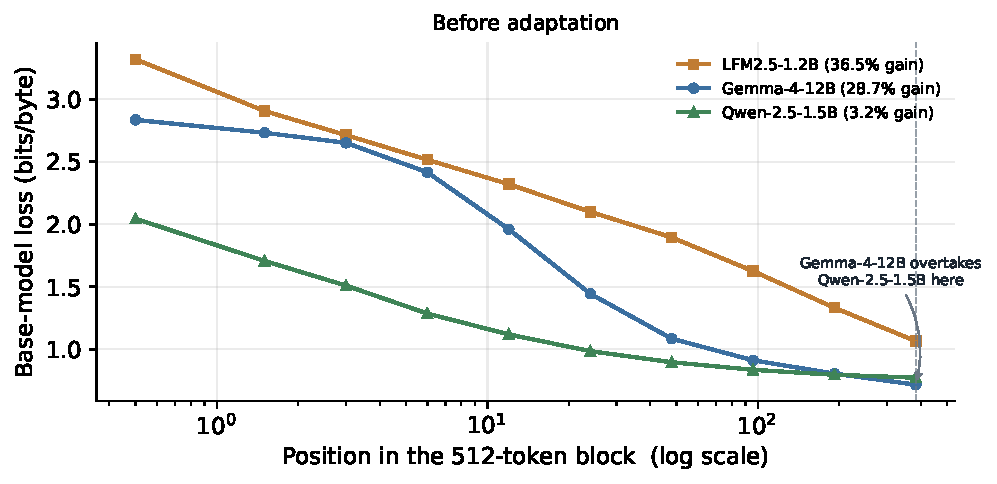
\includegraphics[width=0.90\textwidth]{fig_block_position_slide.pdf}
  \end{column}
  \begin{column}{0.37\textwidth}
    \footnotesize
    Corpus loss is aggregated over independent 512-token blocks, so nearly all cuts start
    mid-document with \emph{no preceding context}.
    \vspace{0em}

    \warmw{The byte-normalized curves cross.} Over the first 8 positions Gemma averages
    2.566 bits/byte vs Qwen's 1.490 --- but at position 256+ Gemma is \goodw{0.717}
    and Qwen \goodw{0.773}.
    \vspace{0em}

    The crossing survives tokenizer normalization: vocabulary size alone does not explain
    it. With context, the 12B model shows the stronger steady-state result.
  \end{column}
  \end{columns}

  \vspace{-0.1em}
  \punch{\scriptsize Among the top 200 gain-carrying tokens: \keyw{`.', `,',
  `\textbackslash n\textbackslash n', ` the', ` and'}. Formatting, punctuation, and
  function words carry 83\% of that mass.}
\end{frame}

% ==================================================================== 10
\begin{frame}
  \frametitle{BPB agrees when tasks measure language}
  \framesubtitle{HellaSwag provides an independent sentence-continuation check}

  \vspace{0.2em}
  \begin{columns}[c]
  \begin{column}{0.56\textwidth}
    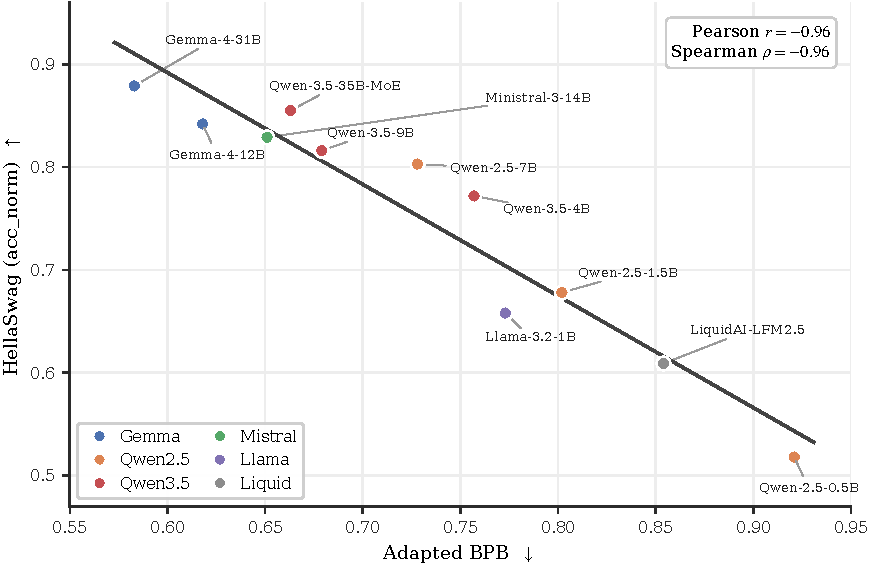
\includegraphics[width=\textwidth]{fig_correlation.pdf}
  \end{column}
  \begin{column}{0.41\textwidth}
    \small
    Adapted \bpb{} vs.\ HellaSwag: \goodw{$r=-0.96$}.
    \vspace{0.7em}

    HellaSwag is sentence \emph{continuation} --- the benchmark closest to plain language
    modelling. There, \bpb{} reproduces it almost exactly.
    \vspace{0.7em}

    The result confirms that \bpb{} tracks language-modelling quality using one corpus we
    control and one unit shared by every model.
    \vspace{0.7em}

    MMLU-Pro and GSM8K then add complementary views of knowledge and arithmetic.
  \end{column}
  \end{columns}
\end{frame}

% ==================================================================== 11
\begin{frame}
  \frametitle{Different tasks reveal different strengths}
  \framesubtitle{\up{n}/\dn{n} $=$ ranks $n$ places higher/lower than \bpb{} puts it}

  \vspace{0.2em}
  \begin{center}
  \renewcommand{\arraystretch}{1.02}
  \scriptsize
  \begin{tabular}{lcccc}
    \toprule
    & \textbf{Adapted \bpb{}} & \textbf{HellaSwag} & \textbf{MMLU-Pro} & \textbf{GSM8K} \\
    \textbf{Model} & \textit{continuation} & \textit{continuation} & \textit{knowledge} & \textit{arithmetic} \\
    \midrule
    Gemma-4-31B        & 1 & 1\same    & 2\dn{1} & 3\dn{2} \\
    Gemma-4-12B        & 2 & 3\dn{1}   & 3\dn{1} & 6\dn{4} \\
    Ministral-3-14B    & 3 & 4\dn{1}   & 5\dn{2} & 5\dn{2} \\
    \rowcolor{wash} Qwen-3.5-35B-MoE   & 4 & 2\up{2}   & 1\up{3} & 1\up{3} \\
    \rowcolor{wash} Qwen-3.5-9B        & 5 & 5\same    & 4\up{1} & 2\up{3} \\
    \rowcolor{wash} Qwen-2.5-7B        & 6 & 6\same    & 6\same  & 4\up{2} \\
    Llama-3.2-1B       & 7 & 7\same    & 9\dn{2} & 9\dn{2} \\
    LiquidAI-LFM2.5    & 8 & 8\same    & 8\same  & 7\up{1} \\
    \rowcolor{wash} Qwen-2.5-0.5B      & 9 & 9\same    & 7\up{2} & 8\up{1} \\
    \midrule
    \textbf{Ranks identical to \bpb{}} & --- & \goodw{6 / 9} & 2 / 9 & \warmw{0 / 9} \\
    \textbf{Largest displacement}      & --- & \goodw{2}     & 3     & \warmw{4} \\
    \bottomrule
  \end{tabular}
  \end{center}

  \vspace{0.3em}
  \footnotesize
  Agreement changes \keyw{monotonically} as the task moves from continuation to knowledge
  to arithmetic. Each column measures a different capability.
\end{frame}

% ==================================================================== 12
\begin{frame}
  \frametitle{The family pattern explains the shift}
  \framesubtitle{GSM8K emphasizes arithmetic strengths learned during pre-training}

  \vspace{0.5em}
  \begin{columns}[t]
  \begin{column}{0.45\textwidth}
    \small
    Every \keyw{Qwen} model ranks \goodw{higher} on GSM8K than in the \bpb{} ordering
    --- $+3, +3, +2, +1$.
    \vspace{0.4em}

    Every \keyw{Gemma / Mistral / Llama} model moves the other way --- $-2, -4, -2, -2$.
    \vspace{0.7em}

    With \keyw{zero exceptions}, the pattern reflects a clear difference in pre-training
    emphasis: GSM8K rewards arithmetic experience.
    \vspace{0.6em}

    \bpb{} keeps \keyw{language modelling} separate from \keyw{arithmetic skill}, so the two
    measurements can be used together.
    \vspace{0.5em}

    {\scriptsize\color{mute} The ninth model, LFM-2.5, also rises one place.}
  \end{column}
  \begin{column}{0.50\textwidth}
    \setlength{\fboxsep}{10pt}
    \colorbox{wash}{\parbox{\dimexpr\textwidth-2\fboxsep\relax}{%
      \small\nohyph
      \textbf{One pair, two capabilities}
      \vspace{0.5em}

      \renewcommand{\arraystretch}{1.15}
      \scriptsize
      \setlength{\tabcolsep}{5pt}
      \begin{tabular}{lcc}
        \toprule
         & \textbf{Qwen-2.5-0.5B} & \textbf{Llama-3.2-1B} \\
        \midrule
        Adapted \bpb{} $\downarrow$ & 0.921 & \textbf{0.773} \\
        HellaSwag $\uparrow$        & 0.518 & \textbf{0.658} \\
        \midrule
        GSM8K $\uparrow$            & \textbf{0.347} & 0.065 \\
        \bottomrule
      \end{tabular}
      \vspace{0.6em}

      Llama is the better language model on both \bpb{} and HellaSwag. On GSM8K the
      0.5B Qwen scores \textbf{5$\times$ higher}.
      \vspace{0.5em}

      The preferred model follows the capability the product needs.
    }}
  \end{column}
  \end{columns}
\end{frame}

% ==================================================================== 13
\begin{frame}
  \frametitle{Adaptation changes the ranking --- then it transfers}
  \framesubtitle{Within-domain reordering; cross-domain stability after adaptation}

  \vspace{-0.15em}
  \begin{center}
    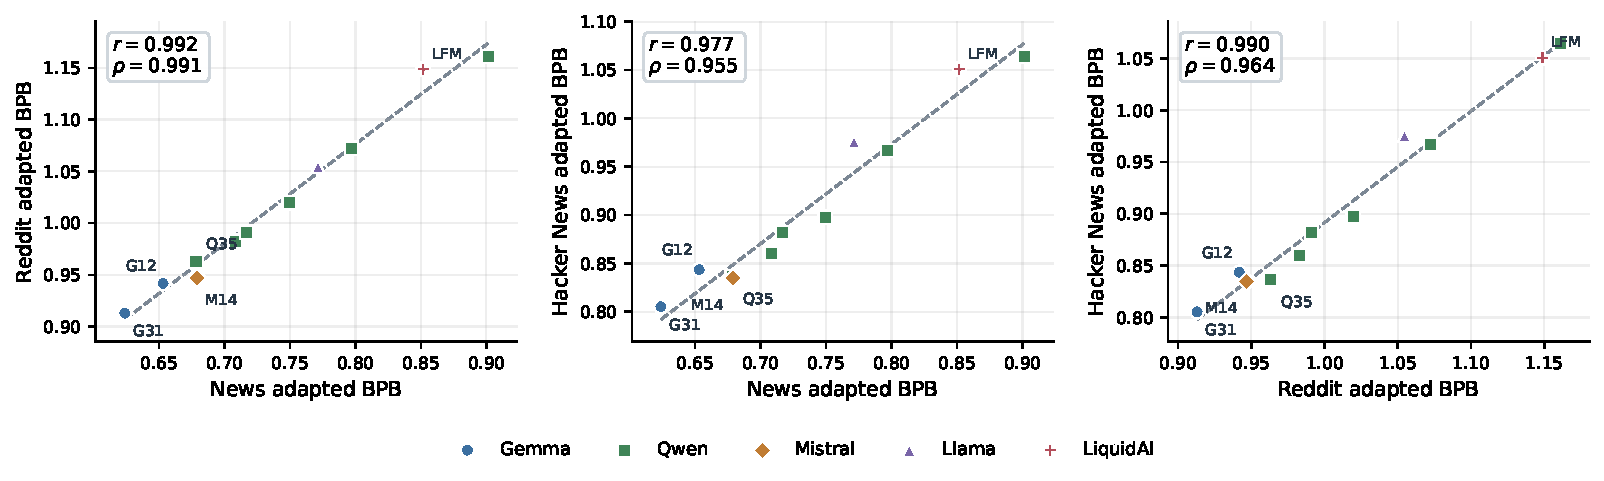
\includegraphics[width=0.90\textwidth]{fig_cross_corpus_slide.pdf}
  \end{center}
  \vspace{-0.55em}
  \begin{columns}[c]
  \begin{column}{0.48\textwidth}
    \footnotesize
    \warmw{Adaptation changes selection:} zero-shot$\rightarrow$adapted
    $\rho=0.655/0.609/0.682$; maximum moves are \textbf{7/7/5 places}.
  \end{column}
  \begin{column}{0.48\textwidth}
    \footnotesize
    \goodw{Adapted ranks transfer:} cross-domain $\rho=+0.991/+0.955/+0.964$;
    no model moves more than two places.
  \end{column}
  \end{columns}
  \vspace{0em}
  \punch{\scriptsize Gemma-4-31B moves from zero-shot rank \textbf{4/5/6} to adapted
  rank \textbf{1/1/1} on news, Reddit, and Hacker News.}
\end{frame}

% ==================================================================== 14
\begin{frame}
  \frametitle{A simple decision rule}

  \vspace{0.9em}
  \small
  \begin{columns}[t]
  \begin{column}{0.47\textwidth}
    \normalsize\textbf{What we learned}\\[0.6em]
    \small
    \begin{itemize}\setlength\itemsep{0.45em}
      \item One coordinate system that is valid across tokenizers and architectures.
      \item Adaptation can change the choice; the adapted ranking remains stable across three corpora.
      \item A 512-token adapter retains its gain through 2{,}048-token inference.
    \end{itemize}
  \end{column}
  \begin{column}{0.47\textwidth}
    \normalsize\textbf{How to use it}\\[0.6em]
    \small
    \begin{itemize}\setlength\itemsep{0.45em}
      \item Collect recent text from the target domain.
      \item Clean and audit it, then adapt every candidate under one budget.
      \item Rank by adapted \bpb{} and test near-ties on the target domain.
    \end{itemize}
  \end{column}
  \end{columns}

  \vspace{0.05em}
  \punch{\footnotesize\textbf{Bottom line:} adapted \bpb{} gives one fair ruler, survives a
  three-domain test, and turns a fresh corpus into a defensible base-model decision.}
\end{frame}

% ==================================================================== 15
{
\setbeamertemplate{footline}{}
\begin{frame}[plain]
  \vspace{2.6em}
  \begin{center}
  {\LARGE\bfseries Thank you}\\[1.0em]
  {\large\color{mute} Questions?}\\[2.2em]
  {\color{rule}\rule{0.5\textwidth}{0.6pt}}\\[1.2em]
  {\small\color{mute} Backup slides follow: full benchmark scores, contamination
  breakdown, adaptation protocol, longer-context transfer.}
  \end{center}
\end{frame}
}

% ==================================================================== 16
\begin{frame}
  \frametitle{Backup: the adaptation results as a table}
  \framesubtitle{Lower \bpb{} is better. The reduction is a calibration diagnostic, not plasticity --- see slide 9.}

  \vspace{0.3em}
  \begin{center}
  \renewcommand{\arraystretch}{1.08}
  \scriptsize
  \begin{tabular}{llrrrr}
    \toprule
    \textbf{Model} & \textbf{Architecture} & \textbf{Params} &
    \textbf{Zero-shot} & \textbf{Adapted} & \textbf{Reduction} \\
    \midrule
    Gemma-4-31B        & Dense Transformer  & 31B   & 0.753 & \textbf{0.583} & 22.6\% \\
    Gemma-4-12B        & Dense Transformer  & 12B   & 0.867 & 0.618 & 28.7\% \\
    Ministral-3-14B    & Dense Transformer  & 14B   & 0.723 & 0.651 & \phantom{0}9.9\% \\
    \rowcolor{wash} Qwen-3.5-35B-MoE   & Mixture of Experts & 35B   & 0.700 & 0.663 & \phantom{0}5.4\% \\
    Qwen-3.5-9B        & Dense Transformer  & 9B    & 0.733 & 0.679 & \phantom{0}7.4\% \\
    Qwen-2.5-7B        & Dense Transformer  & 7B    & 0.753 & 0.728 & \phantom{0}3.3\% \\
    Qwen-3.5-4B        & Dense Transformer  & 4B    & 0.775 & 0.757 & \phantom{0}2.3\% \\
    Llama-3.2-1B       & Dense Transformer  & 1.2B  & 0.814 & 0.773 & \phantom{0}5.1\% \\
    Qwen-2.5-1.5B      & Dense Transformer  & 1.5B  & 0.829 & 0.802 & \phantom{0}3.2\% \\
    \rowcolor{wash} LiquidAI-LFM2.5    & Liquid Neural Net  & 1.2B  & 1.346 & 0.854 & \textbf{36.5\%} \\
    Qwen-2.5-0.5B      & Dense Transformer  & 0.5B  & 0.931 & 0.921 & \phantom{0}1.0\% \\
    \bottomrule
  \end{tabular}
  \end{center}

  \vspace{0.5em}
  \footnotesize
  Every value here reproduces from \texttt{results/summary.json} at full precision.
\end{frame}

% ==================================================================== 17
\begin{frame}
  \frametitle{Backup: the full numbers behind slides 11--12}
  \framesubtitle{The ranks and displacements on slide 11 are derived from this table}

  \vspace{0.3em}
  \begin{center}
  \renewcommand{\arraystretch}{1.08}
  \scriptsize
  \begin{tabular}{lrrrrr}
    \toprule
    \textbf{Model} & \textbf{Adapted \bpb{}} & \textbf{MMLU-Pro} &
    \textbf{HellaSwag} & \textbf{GSM8K} & \textbf{Macro} \\
    \midrule
    Gemma-4-31B      & \textbf{0.583} & 0.612 & \textbf{0.865} & 0.817 & 0.764 \\
    Gemma-4-12B      & 0.618 & 0.583 & 0.840 & 0.778 & 0.733 \\
    Ministral-3-14B  & 0.651 & 0.541 & 0.829 & 0.807 & 0.726 \\
    Qwen-3.5-35B-MoE & 0.663 & \textbf{0.620} & 0.855 & \textbf{0.865} & \textbf{0.780} \\
    Qwen-3.5-9B      & 0.679 & 0.562 & 0.816 & 0.860 & 0.746 \\
    Qwen-2.5-7B      & 0.728 & 0.475 & 0.803 & 0.813 & 0.697 \\
    Llama-3.2-1B     & 0.773 & 0.117 & 0.658 & 0.065 & 0.280 \\
    LiquidAI-LFM2.5  & 0.854 & 0.155 & 0.609 & 0.550 & 0.438 \\
    Qwen-2.5-0.5B    & 0.921 & 0.167 & 0.518 & 0.347 & 0.344 \\
    \bottomrule
  \end{tabular}
  \end{center}

  \vspace{0.5em}
  \footnotesize
  Rank analysis uses the nine-model common subset reported across \bpb{} and all three tasks. Harness:
  \emph{lm-evaluation-harness}, vLLM backend, bf16, greedy decoding, each tokenizer's
  native BOS. MMLU-Pro 5-shot CoT on a fixed 1{,}000-question subset; HellaSwag 10-shot
  length-normalized; GSM8K 5-shot flexible-extract.
\end{frame}

% ==================================================================== 18
\begin{frame}
  \frametitle{Backup: contamination breakdown}
  \framesubtitle{$N=1000$ sampled sequences per model; 80 unique global leaks removed}

  \vspace{0.3em}
  \begin{center}
  \renewcommand{\arraystretch}{1.08}
  \scriptsize
  \begin{tabular}{lrrrrr}
    \toprule
    \textbf{Model} & \textbf{Min-K++ flags} & \textbf{CoDeC flags} &
    \textbf{DCQ candidates} & \textbf{DCQ acc.} & \textbf{Verified leaks} \\
    \midrule
    google-gemma-4-31B        & 12 & 6 & 20 & 100\% & 20 \\
    google-gemma-4-12B        & 11 & 6 & 11 & 100\% & 11 \\
    mistralai-Ministral-3-14B & 12 & 8 & 13 & 100\% & 13 \\
    Qwen-Qwen3.5-35B-MoE      & \phantom{0}6 & 8 & 11 & 100\% & 11 \\
    Qwen-Qwen3.5-9B           & 12 & 6 & 17 & 100\% & 17 \\
    Qwen-Qwen2.5-7B           & 10 & 6 & 14 & 100\% & 14 \\
    Qwen-Qwen3.5-4B           & \phantom{0}9 & 6 & 12 & 100\% & 12 \\
    meta-llama-Llama-3.2-1B   & 17 & 0 & 28 & 100\% & 28 \\
    Qwen-Qwen2.5-1.5B         & 14 & 4 & 17 & 100\% & 17 \\
    LiquidAI-LFM2.5           & 12 & 8 & 23 & \phantom{0}96\% & 22 \\
    Qwen-Qwen2.5-0.5B         & \phantom{0}8 & 2 & 13 & 100\% & 13 \\
    \bottomrule
  \end{tabular}
  \end{center}

  \vspace{0.5em}
  \small Model size does \emph{not} linearly predict memorization --- Llama-3.2-1B
  leaks most in this cohort.
\end{frame}

% ==================================================================== 19
\begin{frame}
  \frametitle{Backup: adaptation protocol}

  \vspace{0.6em}
  \footnotesize
  \begin{columns}[t]
  \begin{column}{0.47\textwidth}
    \textbf{Data handling}
    \begin{itemize}\setlength\itemsep{0.3em}
      \item Google News slice, 8 June 2026: 119{,}054 articles, $\sim$361\,MB.
      \item 80/10/10 train/val/test, seed 42, enforced zero intersection between splits.
      \item Packed into contiguous 512-token blocks along EOS boundaries.
    \end{itemize}
    \vspace{0.9em}
    \textbf{Scoring}
    \begin{itemize}\setlength\itemsep{0.4em}
      \item Corpus-wide cross-entropy over independent 512-token test blocks.
      \item Context resets at block cuts; injected start markers are context, not targets.
      \item Model-specific bytes-per-token factor estimated from the test text.
    \end{itemize}
  \end{column}
  \begin{column}{0.47\textwidth}
    \textbf{Per-model HPO}
    \begin{itemize}\setlength\itemsep{0.4em}
      \item 20-trial Optuna sweep, Successive Halving (top 33\% promoted).
      \item LoRA rank $r\in\{8,16,32,64\}$; $\alpha$-multiplier $\in\{1,2,4\}$;
      dropout; LR $10^{-6}$--$10^{-3}$ log-scale; effective batch to 128 via
      gradient accumulation.
      \item Adapters restricted to the language backbone.
      \item Winner trained to convergence: cosine schedule to $0.1\times$ peak LR,
      gradient clip 1.0.
    \end{itemize}
    \vspace{0.4em}
    Hardware: A100/H100 multi-node under Slurm.
  \end{column}
  \end{columns}
\end{frame}

% ==================================================================== 20
\begin{frame}
  \frametitle{Backup: 512-token adaptation transfers to longer contexts}
  \framesubtitle{Same held-out targets; only the available preceding context changes}

  \vspace{-0.1em}
  \begin{center}
    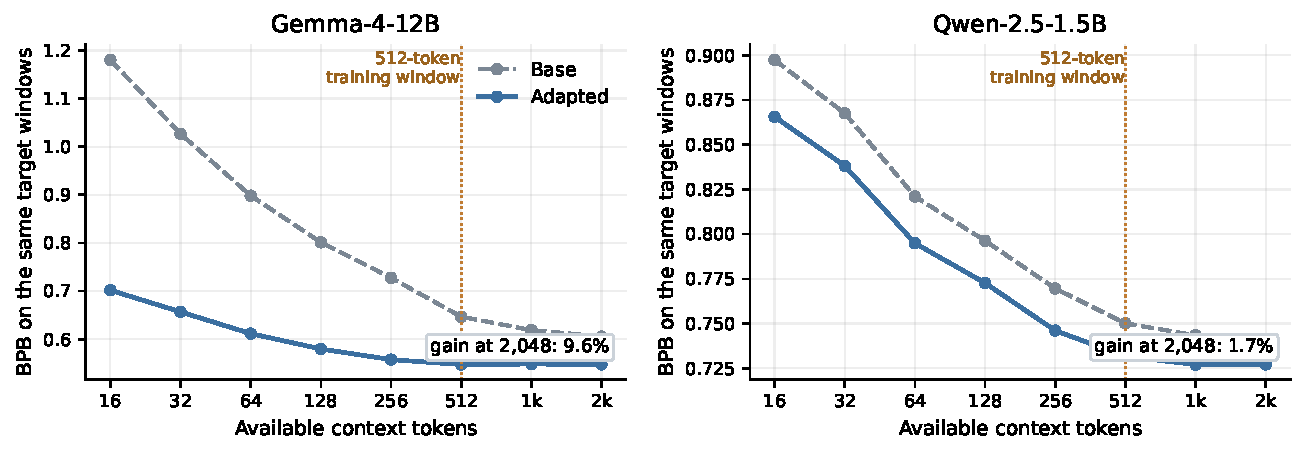
\includegraphics[width=0.82\textwidth]{fig_context_length_slide.pdf}
  \end{center}
  \vspace{-0.35em}
  \begin{columns}[c]
  \begin{column}{0.48\textwidth}
    \footnotesize
    Gemma base BPB keeps recovering after 512: \textbf{0.6465 $\rightarrow$ 0.6054} at
    2{,}048 tokens.
  \end{column}
  \begin{column}{0.48\textwidth}
    \footnotesize
    Adapted Gemma stays at \textbf{0.547}; its advantage remains \goodw{9.6\%} at
    four times the training context.
  \end{column}
  \end{columns}
  \vspace{0.05em}
  \punch{\scriptsize The adapter does not require the inference sequence to stop at 512 tokens.}
\end{frame}

\end{document}
